\documentclass{article}
\usepackage{physics}
\usepackage{graphicx}
\usepackage{caption}
\usepackage{amsmath}
\usepackage{authblk}
\usepackage{amsfonts}
\usepackage{esint}
\usepackage{mathtools}
\usepackage{amsthm}
\theoremstyle{definition}
\newtheorem{defn}{Definition}[section]
\newtheorem{prop}{Proposition}[section]
\newtheorem{rmk}{Remark}[section]
\newtheorem{exmp}{Example}[section]
\newtheorem{prob}{Problem}[section]
\newtheorem{sln}{Solution}[section]
\newtheorem*{prob*}{Problem}
\newtheorem*{sln*}{Solution}
\usepackage{empheq}
\usepackage{hyperref}
\usepackage{tensor}
\usepackage{xcolor}
\hypersetup{
	colorlinks,
	linkcolor={black!50!black},
	citecolor={blue!50!black},
	urlcolor={blue!80!black}
}
\newcommand{\p}{\partial}
\newcommand{\R}{\mathbb{R}}
\newcommand{\lag}{\mathcal{L}}


\begin{document}
\begin{titlepage}\centering
 \clearpage
 \title{\textsc{\bf{PARTIAL\\ DIFFERENTIAL EQUATIONS}}\\\smallskip A Quick Guide\\}
 \author{\bigskip Huan Q. Bui}
 \affil{Colby College\\Physics \& Statistics\\Class of 2021\\}
 \date{\today}
 \maketitle
 \thispagestyle{empty}
\end{titlepage}

\subsection*{Preface}
\addcontentsline{toc}{subsection}{Preface}

Greetings,\\

\textit{Partial Differential Equations: A Quick Guide} is based on my lecture notes from MA411: Topics in Differential Equations - Partial Differential Equations with professor Evan Randles at Colby. The contents are somewhat based on Farlow's \textit{Partial Differential Equations for Scientists and Engineers}.\\	

Enjoy!

\newpage
\tableofcontents
\newpage

\section{Overview and Classification}

%\date{Feb 6, 2019}


\subsection{What in the world is a PDE?}
We shall begin with what PDEs are. 
\begin{defn}
	A partial differential equation (PDE) is an equation relating a function of several variables $\psi(t,\vec{x})$ to its partial derivatives: $\partial_{x_1}\psi$, $\partial^2_{x_1x_2}\psi$, etc.\\
	
	A note on notation:
	\begin{align*}
	\frac{\partial^2 \psi}{\partial x_1\,\partial x_2} \equiv \partial^2_{x_1x_2}\psi \equiv \partial_{x_1}\partial_{x_2}\psi.
	\end{align*}
\end{defn}

\subsection{Some notable examples}
Let us look at a couple of famous PDEs:
\begin{exmp}
	\textbf{Laplace Equation:}
	\begin{align*}
	\Delta \psi = \nabla^2\psi = \frac{\partial^2 \psi}{\partial x^2} + \frac{\partial^2 \psi}{\partial y^2} + \frac{\partial^2 \psi}{\partial z^2} = 0.
	\end{align*}
\end{exmp}

\begin{exmp}
	\textbf{Poisson's Equation:}
	\begin{align*}
	\Delta \psi = \nabla^2 \psi = F(x,y,z)
	\end{align*}
\end{exmp}

We take note of the \textbf{Laplacian} or the \textbf{Laplacian operator}:
\begin{align*}
\boxed{\Delta \psi \equiv \nabla^2 \psi = \frac{\partial^2 \psi}{\partial x^2} + \frac{\partial^2 \psi}{\partial y^2} + \frac{\partial^2 \psi}{\partial z^2}}
\end{align*}
The Laplacian operator takes a function $\psi$ linearly to another function $\nabla^2 \psi$. The Laplacian is one of the most important objects in mathematics, as it touches probability theory, potential theory, partial differential equations, mathematical physics, harmonic analysis, number theory, etc.\\

Another note on notation: the symbols $\Delta$ and $\nabla^2$ will be used interchangeably in this text. The $\nabla^2$ represents the divergence of the gradient.\\

Let us look at some more examples to see the ubiquity of the Laplacian in PDEs:
\begin{exmp}
	\textbf{The heat equation:}
	\begin{align*}
	\frac{\partial \psi}{\partial t} = \nabla^2 \psi.
	\end{align*}
	The heat equation describes heat transfer over time. But there is also a connection between the heat equation and probability theory. In particular, the Gaussian function:
	\begin{align*}
	\frac{1}{\sqrt{4\pi t}}e^{-\frac{x^2}{4t}}
	\end{align*}
	solves the heat equation.
\end{exmp}

\begin{exmp}
	\textbf{The wave equation:}
	\begin{align*}
	\frac{\partial^2 \psi}{\partial t^2} = \nabla^2 \psi.
	\end{align*}
	The wave equation describes physical vibrations. The second $t$-derivative in the equation is strongly correlated to Newton's second law of motion.
\end{exmp}

\begin{exmp}
	\textbf{The Schr\"{o}dinger equation:}
	\begin{align*}
	i\hbar \frac{\partial \psi}{\partial t} = -\frac{\hbar^2}{2m}\nabla^2\psi + V(t,\vec{x})\psi.
	\end{align*}
	One can hardly talk about PDEs without mentioning the Schr\"{o}dinger equation. There is a strong resemblance between the Schr\"{o}dinger equation and the wave equation. Of course, this is no coincidence, as the Schr\"{o}dinger equation is postulated based on a description of a harmonic oscillator.  
\end{exmp}

Our next example does not include the Laplacian operator. 

\begin{exmp}
	\textbf{The telegraphic equation:}
	\begin{align*}
	\frac{\partial^2 \psi}{\partial t^2} = \frac{\partial^2 \psi}{\partial x^2} + \alpha \frac{\partial \psi}{\partial t} + \beta \psi.
	\end{align*}
	The telegraphic equation describes the transfer of information. 
\end{exmp}

\subsection{Vocabulary}
\begin{itemize}
	\item The function $\psi$ appearing in a given PDE is called the ``dependent variable.''
	\item The variables $t,x_1,x_2,\dots$ are called ``independent variables.''
\end{itemize}

\subsection{Our goals}
Our goal is, given a PDE, to find a sufficiently differentiable function which satisfies it that is subject to \textbf{boundary} and \textbf{initial} conditions. 

\subsection{Our plan}
Here are the key concepts we will explore in this text:
\begin{itemize}
	\item Modeling: Formulate same physical problem in terms of PDEs.
	\item Learn how to solve (some) PDEs, subjection to initial conditions and boundary conditions. This means we will be looking at ideas like:
	\begin{itemize}
		\item Separation of variables, in order to reduce a PDE into a system of ODEs.
		\item Integral transforms, in order to reduce the number of independent variables.
		\item Change of coordinates, in order to change a complicated PDE into another one which is easier to solve.
		\item Eigenfunction expansion, which generally goes under the Sturm-Liouville theory.
		\item Numerical methods, as most PDEs cannot be solved analytically. 
	\end{itemize}
\end{itemize}

\subsection{Classification}
\begin{itemize}
	\item The order of a PDE is the highest order of partial derivatives appearing (non-trivially) in the PDE.
	\begin{exmp}
		\begin{align*}
		\frac{\partial \psi}{\partial t} = \nabla^2\psi
		\end{align*}
		is a second-order PDE.
	\end{exmp}
	\begin{exmp}
		\begin{align*}
		\frac{\partial \psi}{\partial t} = \partial^4_x\psi
		\end{align*}
		- the biharmonic heat equation, is a fourth-order PDE.
	\end{exmp}
	\item Linearity: A PDE is linear if the function $\psi$ and its derivatives appear in a linear way.
	\begin{exmp}
		All second-order linear PDEs in 2 variables are of the form:
		\begin{align*}
		\boxed{A\frac{\partial^2 \psi}{\partial x^2} + B\frac{\partial^2 \psi}{\partial x\,\partial y} + C\frac{\partial^2 \psi}{\partial y^2} + D\frac{\partial \psi}{\partial x} + E\frac{\partial \psi}{\partial y} + F\psi = G}
		\end{align*}
	\end{exmp}
\end{itemize}

% Feb 08, 2019

Note: define
\begin{align*}
L[\psi](x,y) = A\frac{\partial^2 \psi}{\partial x^2} + B\frac{\partial^2 \psi}{\partial x\,\partial y} + C\frac{\partial^2 \psi}{\partial y^2} + D\frac{\partial \psi}{\partial x} + E\frac{\partial \psi}{\partial y} + F\psi
\end{align*}
then we get
\begin{align*}
L[u] = G.
\end{align*}
We get a linear map $L:\psi\rightarrow L[\psi]$. So, for $\gamma, \sigma \in \mathbb{R}$
\begin{align*}
L[\gamma u+ \sigma v)] = \gamma L[u] + \sigma L[v].
\end{align*}
This observation justifies the moniker ``linear.'' Next, we say that $L[\psi] = G$ is \textbf{homogeneous} if $G = 0$. The equation is \textbf{inhomogeneous} if $G(x,y)\neq 0$ for some $x,y$.\\

If $A,B,C,D,E,F$ are constants, then $L[\psi] = G$ is said to be a \textbf{constant-coefficient} equation. Otherwise (at least one of $A,B,C,D,E,F$ is a function of $x,y$ in some non-trivial way), it is said to have \textbf{variable coefficients}. 

\begin{exmp}
	Classify: $u_t = \sin t u_{xx}$.\\
	
	It is a linear PDE, $A = \sin t$, $B=C=D=F=0$, $E=-1$, $G=0$, variable coefficient, and homogeneous. 
\end{exmp}
\begin{exmp}
	Classify: $u_{xx} -\sin u = 0$.\\
	
	Not linear.
\end{exmp}

\begin{exmp}
	Classify: $xu_x - yu_y = 0$.\\
	
	First-order homogeneous linear PDE with variable coefficients. 
\end{exmp}

Note: Linear PDEs are quite well understood. Notable mathematicians who established theories of linear PDEs: Ehenpres(?), Hille, Browder, Soboher, Nash, Nierenburd, Friedmann, Schwartz, Hormander (Fields, 1962), Gardiy.\\

Note: Constant coefficient equations are \textbf{much easier} to solve than variable coefficient equations, because Fourier analysis makes a lot of the constant coefficient problems easy.\\

Note: Non-linear equations are really hard, and there is no general theory. Each type of non-linear problem demands its own special techniques (well, if they exist at all). 

\subsection{Types of second order linear PDE}
\textbf{Parabolic:} $L[\psi] = G$ is said to be parabolic if $B^2 - 4AC = 0$ ($A,B,C$ don't have to be constant coefficients - so the PDE can be parabolic in some region and not elsewhere). 
\begin{exmp}
	The heat equation
	\begin{align*}
	u_t = u_{xx}
	\end{align*}
	is a parabolic equation, because $A=1, E=-1, B=C=0$. 
\end{exmp}

\textbf{Elliptic:} $L[\psi] = G$ is elliptic if $B^2 - 4AC < 0$.
\begin{exmp}
	Laplace's equation
	\begin{align*}
	\delta u = u_{xx} + u_{yy} = 0
	\end{align*}
	is elliptic, because $A=C=1, B=0$.
\end{exmp}

\textbf{Hyperbolic: } if $B^2 - 4AC > 0$.
\begin{exmp}
	The wave equation:\begin{align*}
	u_{tt} = u_{xx}
	\end{align*}
	is hyperbolic, because $B=0, A=1, C=-1$.
\end{exmp}

\newpage

\subsection{Lesson 1: Selected Problems \& Solutions}
\begin{prob*}[\textbf{3}]
	If $u_1(x,t)$ and $u_2(x,t)$ satisfy $L[u] = G$, then is it true that the sum satisfies it? If yes, show.
	\begin{sln*}[\textbf{3}]
		Yes. We have established, in class, that if we define $L : u \rightarrow L[u]$ where  
		\begin{align*}
		L[u] = Au_{xx} + Bu_{xt} + Cu_{tt} + Du_x + Eu_t + Fu = G,
		\end{align*}
		then $L[u]$ is a linear map, which can be readily shown:
		\begin{align*}
		L[\mu u_1 + \nu u_2 ] &= \mu(Au_{1xx} + Bu_{1xt} + Cu_{1tt} + Du_{1x} + Eu_{1t} + Fu_1) \\
		&\text{ }\,\,\,\,\,\,\,+\nu(Au_{2xx} + Bu_{2xt} + Cu_{2tt} + Du_{2x} + Eu_{2t} + Fu_2)\\
		&= \mu L[u_1] + \nu L[u_2].
		\end{align*}
		So, the sum of $u_1$ and $u_2$ also satisfies $L[u] = G$.
	\end{sln*}
\end{prob*}

\begin{prob*}[\textbf{4}]
	Probably the easier of al PDEs to solve is the equation
	\begin{align*}
	\frac{\partial u(x,y)}{\partial x} = 0.
	\end{align*}
	Can you solve this equation? Find all functions $u(x,y)$ that satisfy it.
	\begin{sln*}[\textbf{4}]
		The PDE suggests that $u$ does not depend on $x$. This means that $u(x,y)$ is just some function of $y$, i.e. $u(x,y) = \tilde{u}(y)$. 
	\end{sln*}
\end{prob*}

\begin{prob*}[\textbf{5}]
	What about the PDE
	\begin{align*}
	\frac{\partial^2 u(x,y)}{\partial x\,\partial y} = 0?
	\end{align*}
	Can you find all solutions $u(x,y)$ to this equation? How many are there? How does this compare with an ODE like
	\begin{align*}
	\frac{d^2 y}{d x^2} = 0
	\end{align*}
	insofar as the number of solutions is concerned?
	\begin{sln*}[\textbf{5}]
		This PDE is a first-order, linear, homogeneous PDE with $B = 1, A=C=D=E=F=0$. Since $B^2 - 4AC = 1 > 0$, the PDE is \textbf{hyperbolic}. The PDE suggests that $u_y$ has no $x$-dependence. From the previous problem, we know that $u_y = f'(y)$. Taking the antiderivative with respect to $y$, we get
		\begin{align*}
		\boxed{u(x,y) = \int f'(y)\,dy = f(y) + g(x)}.
		\end{align*} 
		Since the variables $x,y$ are exchangeable (by the equality of mixed partials), following the same argument starting with $u_x$ gives the same form for $u(x,y)$.\\
		
		\noindent The ODE $D^2[y] = y''(x) = 0$ is a second-order, linear, homogeneous ODE. We know that the solution space has dimension of 2:
		\begin{align*}
		\ker(D^2) = \span \{ 1, x \}.
		\end{align*} 
		So while there are infinitely many solutions, only \textbf{two} linearly independent solutions are sufficient to generate all solutions. Whereas there are infinitely many linearly independent solutions to the PDE. We can simply generate a new (linearly independent from $f(y) + g(x)$) solution by multiplying $f(y)$ by $y$ or $g(x)$ by $x$. 
	\end{sln*}
\end{prob*}

\newpage


\section{Diffusion-type problems (parabolic equations): A study of the heat equation}
\subsection{An experiment}
We consider a copper rod of length $L$, which allows heat to transfer along the rod, but is insulated in such a way that heat does not transfer laterally across/out of the rod. 
\begin{figure}[h!]
	\centering
	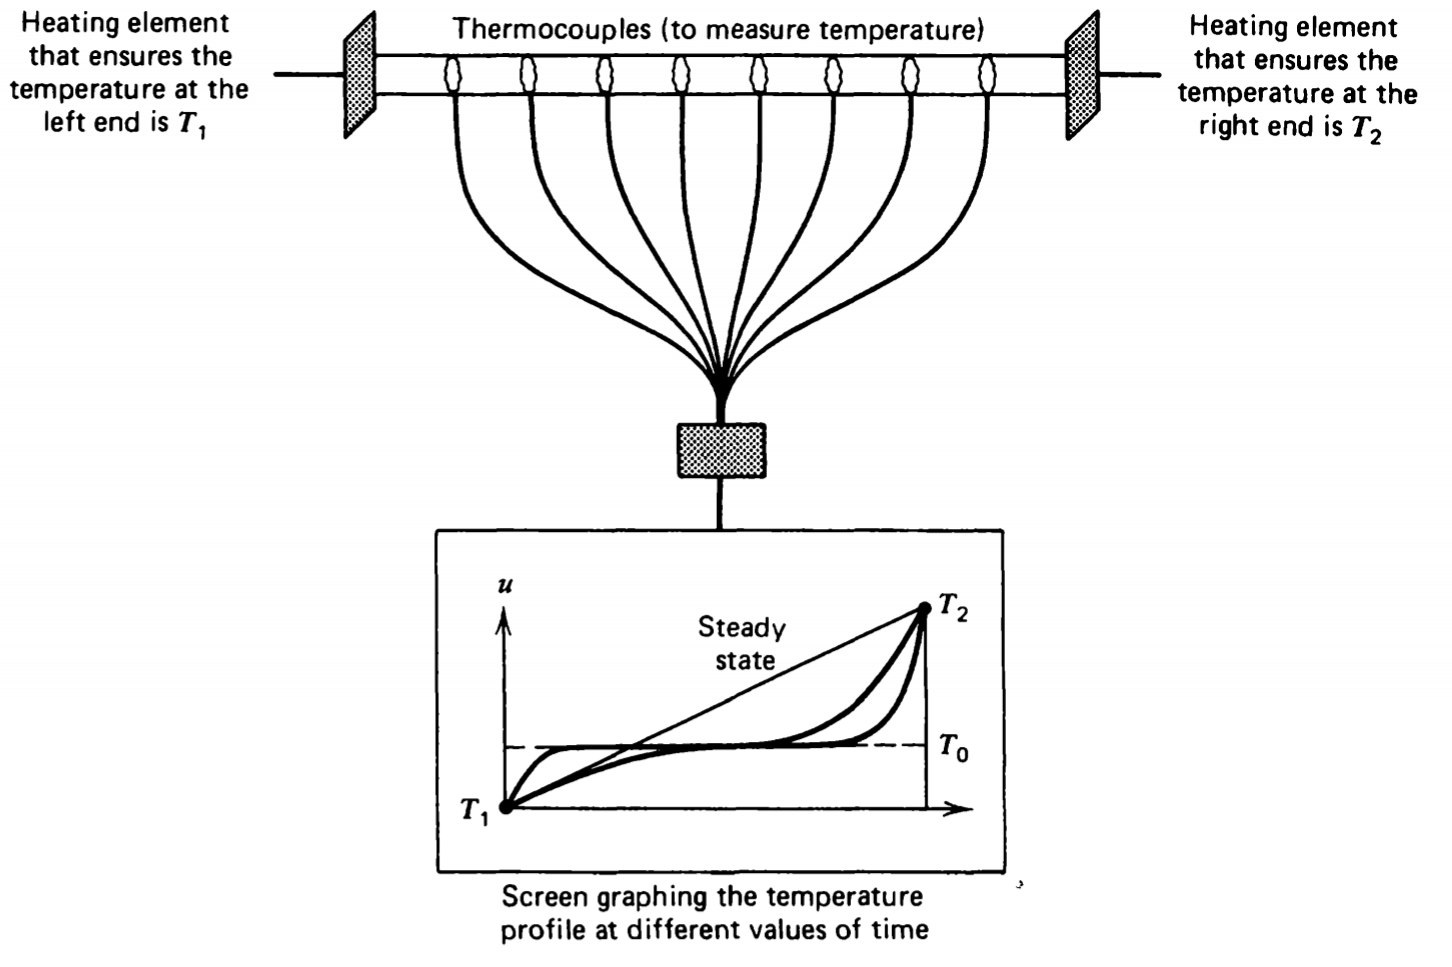
\includegraphics[scale=0.5]{copper.png}
\end{figure}

At time $t=0$, the temperature in the rod is known.
\begin{align*}
u(0,x) = T_0
\end{align*}
The ends of the rod are placed in thermal baths which hold their temperatures fixed. So, at $x=0$, $u(t,0) = T_1$ and at $x=L$, $u(t,L) = T_2$ for all $t>0$.
\subsection{The Mathematical Model}
This behavior is modeled by the heat equation. 
\begin{align*}
u_t = \alpha^2 u_{xx},
\end{align*}
where $\alpha \in \mathbb{R}$, determined by the thermo-character of the rod. $u_t$ is the rate of change of temperature in time, and $u_{xx}$ is the concavity profile in space. \\

Some justification for the heat equation: we look at the spatial difference quotient. For small change in $x$, $\Delta x$:
\begin{align*}
u_{xx} &\approx \frac{u_x(t,x+\Delta x) - u_x(t,x)}{\Delta x}\\
&\approx \frac{(u(t,x+\Delta x) - u(t,x))/\Delta x - (u(t,x)-u(t,x-\Delta x))/\Delta x}{\Delta x}\\
&\approx \frac{1}{\Delta x^2}(u(t,x+\Delta x) + u(t,x-\Delta x) - 2u(t,x))\\
&\approx \frac{2}{\Delta x^2}\left(\frac{u(t,x+\Delta x) + u(t,x-\Delta x)}{2} - u(t,x) \right)
\end{align*}
So, $u_{xx} \propto$ the difference between the average temperatures among neighboring points and the temperature at $x$. 
\begin{figure}[h!]
	\centering
	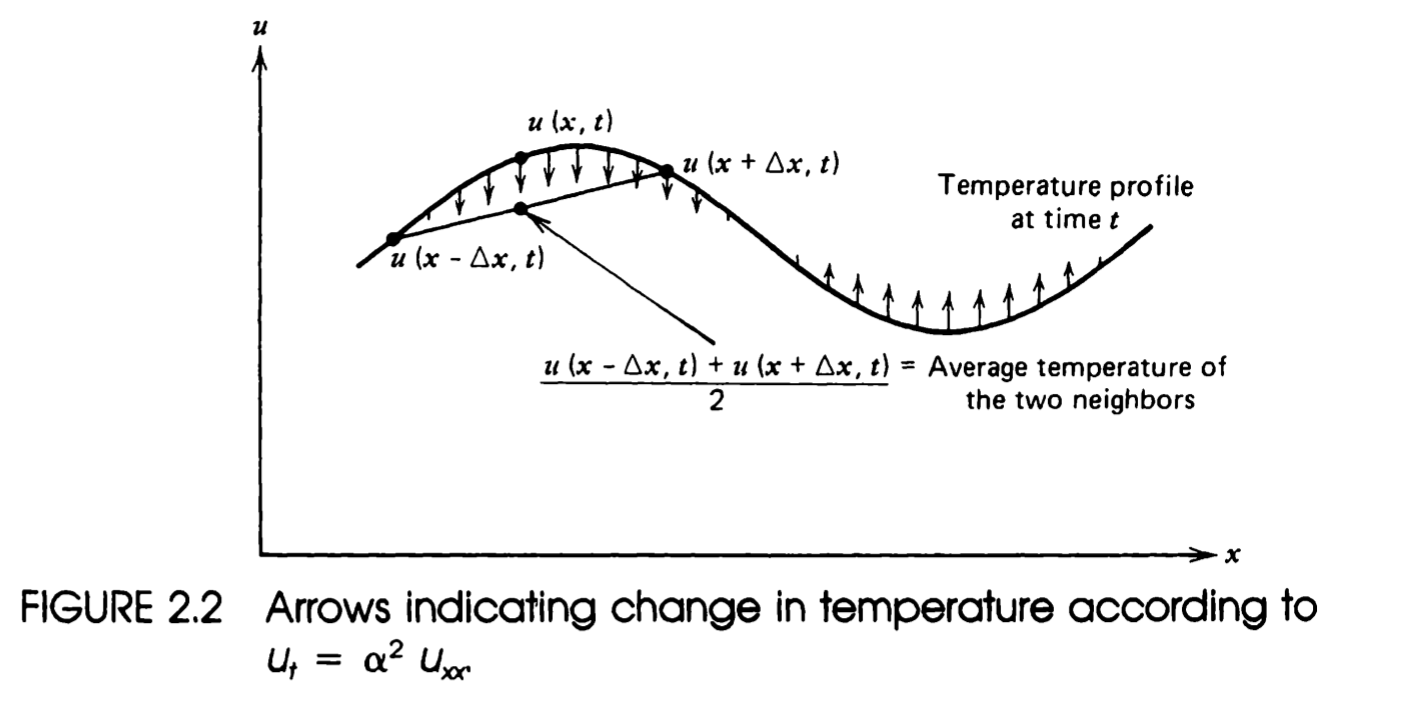
\includegraphics[scale=0.5]{copper1.png}
\end{figure}

Assume that $u_t = \alpha^2 u_{xx}$, then if $u_{xx} < 0$, then $u_t < 0$, i.e. temperature decreases in time. If $u_{xx} > 0$, then $u_t > 0$, i.e. temperature increases in time. If $u_{xx} = 0$, the temperature stays fixed. 

% Feb 11, 2019
\subsection{Boundary Conditions}
In contrast to ODEs, PDE have different types of constraints which are combined with the PDE to form well-posed problems, where ``well-posed'' means that a unique solution exists. Our conditions are often (and will almost always) be physically motivated. \\

Let us revisit the heat equation. 
\begin{align*}
u_t = \alpha^2 u_{xx}, t> 0, 0\leq x\leq L.
\end{align*}
The temperatures at the ends $x=0$ and $x=L$ are fixed $T_1$ and $T_2$ by the thermal baths, so the boundary conditions are
\begin{align*}
BCs = \begin{cases*}
u(0,t) = T_1\\
u(L,t) = T_2
\end{cases*}
\forall t > 0.
\end{align*} 
Here ``boundary'' refers to the boundary of $[0,L]$.
\subsection{Initial Conditions}
Our problem also involves evolution in time, we have an initial condition of the form
\begin{align*}
u(x,0) = T_0 \text{ or } u(x,0) = u_0(x) \forall x \in [0,L]
\end{align*}
where $T_0$ is the initial constant temperature of the rod and $u_0(x)$ is the initial temperature which is allowed to vary (some spatial distribution). All together, we form an initial boundary value problem, an IBVP of the form
\begin{align*}
\begin{cases*}
u_t = \alpha^2 u_{xx}, t>0,x\in[0,L]\\
u(0,t) = T_1, \forall t > 0\\
u(L,t) = T_2,\forall t > 0\\
u(x,0) = T_0, \forall x\in[0,L]
\end{cases*} 
\end{align*}
\subsection{A Couple of Variants}
\subsubsection{Lateral Heat Loss}
This allows for heat to be transferred laterally into the rod according to Newton's law of cooling. So the new heat equation is
\begin{align*}
u_t = \alpha^2 u_{xx} -\beta(u - u_0), \beta > 0
\end{align*}
where $u_0$ is the outside temperature.
\subsubsection{Internal Heat Source}
If, by some non-diffusive heat source, heat is added into the rod at $(t,x)$, the equation is
\begin{align*}
u_t = \alpha^2 u_{xx} + f(x,t)
\end{align*}
where $f(x,t)$ is the heat added to the rod, internally. This PDE is \textit{inhomogeneous}.
\subsubsection{Diffusion-convection Equation}
\begin{align*}
u_t = \alpha^2 u_{xx} - vu_x
\end{align*}
If $u$ describes the amount (not heat) pollutant, then the term $-vu_x$ describes the flow of additional pollutant introduced by the moving particles. 
\subsubsection{Variable-coefficients case}
When the thermal make up of the rod (its thermal character) is allowed to vary according to a variable diffusivity coefficient, i.e. $\alpha \rightarrow \alpha(x)$, then the relevant heat equation is
\begin{align*}
u_t = \alpha^2(x)u_{xx}.
\end{align*}
So, let's say
\begin{align*}
\alpha(x) = 
\begin{cases*}
\alpha_{Copper}, x\in[0,L/2]\\
\alpha_{Bronze}, x\in[L/2,L]
\end{cases*}
\end{align*}
\subsection{Other types of Boundary Conditions}
\subsubsection{Type 1}
Let's revisit the original heat equation: $u_t = \alpha^2 u_{xx}$. If we force the rod ends to have time-dependent temperatures: $g_1(t)$ and $g_2(t)$ at $x=0$ and $x=L$ respectively, then our boundary conditions are
\begin{align*}
BCs = 
\begin{cases*}
u(0,t) = g_1(t)\\
u(L,t) = g_2(t)
\end{cases*}
\forall t > 0.
\end{align*} 
If instead we're studying the heat flow on a circular plate, i.e., where $u = u(t,t,\theta)$, and the heat EQ is 
\begin{align*}
u_t = \alpha^2 \nabla^2 u = \alpha^2\left( u_{rr} + \frac{1}{r}u_r + \frac{1}{r^2}u_{\theta\theta} \right).
\end{align*}
Here, the boundary conditions look like $u(t,r_0,\theta) = g(t,\theta)$, i.e. we force the disk to have temperature $g(t,\theta)$ along the boundary.
\subsubsection{Type 2 (more realistic)}
We take into account heat transfer to rod ends via thermal bath. Suppose that our rod is placed in bath (liquid) at each end of temperature $g_1(t)$ and $g_2(t)$ respectively. 
\begin{figure}[h!]
	\centering
	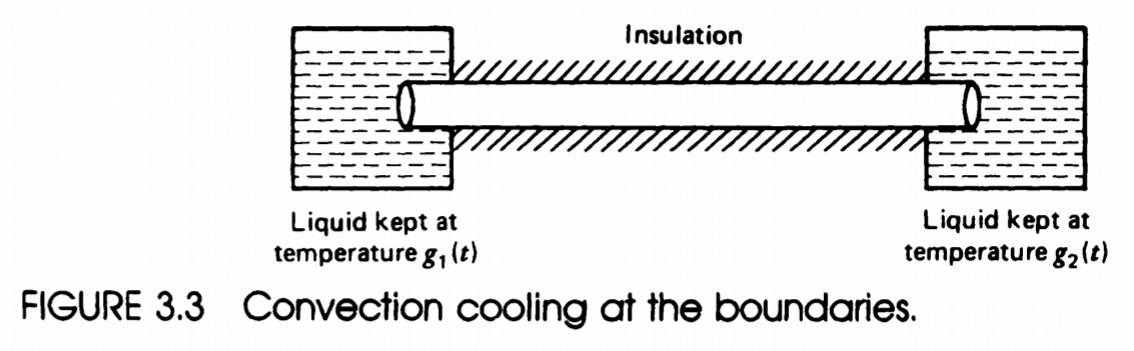
\includegraphics[scale=0.7]{type2.png}
\end{figure}

In view of Newton's law of cooling, the heat flux at a rod end is $h(u(t,0) - g_(1))$ at $x=0$ and $h(u(t,L)-g_2(t))$ at $x=L$, and $h$ is some constant. Next, we introduce Fourier's law of heat flux (empirical):
\begin{align*}
\frac{\p u}{\p n} = k \times\text{Heat flux}
\end{align*}
where $n$ is the \textit{inward normal} direction to the boundary, and $k\in\R$. At $x=0$:
\begin{align*}
\begin{cases*}
\frac{\p u}{\p n} = u_x(t,0) = kh(u(t,0)-g_1(t)), x=0\\
\frac{\p u}{\p n} = -u_x(t,L) = kh(u(t,L)-g_2(t)), x=L
\end{cases*}.
\end{align*}
So, the BC for Type 2 is the following
\begin{align*}
\begin{cases*}
u_x(t,0) = kh(u(t,0) - g_1(t))\\
u_2(t,L) = -kh(u(t,L) - g_2(t))
\end{cases*}
\end{align*}
The 2-D plate analogue is the following. We require (since $r$ is outward)
\begin{align*}
-\frac{\p u}{\p r} = -kh(u(t,r_0,\theta) - g(t,\theta))
\end{align*}
where $g(t,\theta)$ is the temperature of the bath surrounding the plate. 


\subsubsection{Type 3: Flux specified - including isolated boundaries} 
The rod ends are insulated, i.e., no heat flows in or out of the rod ends. So the boundary conditions are
\begin{align*}
u_x(0,t) = u_x(L,t) = 0 \forall 0 < t < \infty.
\end{align*}
In two variables (a disk), the analogous BC is
\begin{align*}
u_r(t,r_0,\theta) = 0 \forall 0 < t < \infty, 0\leq \theta \leq 2\pi.
\end{align*}
\subsubsection{Type 4: Mixed}
We can mix BCs. Suppose that one end of the rod has zero flux condition (type 3) and the other end is submerged in a liquid (type 2).

\begin{figure}[h!]
	\centering
	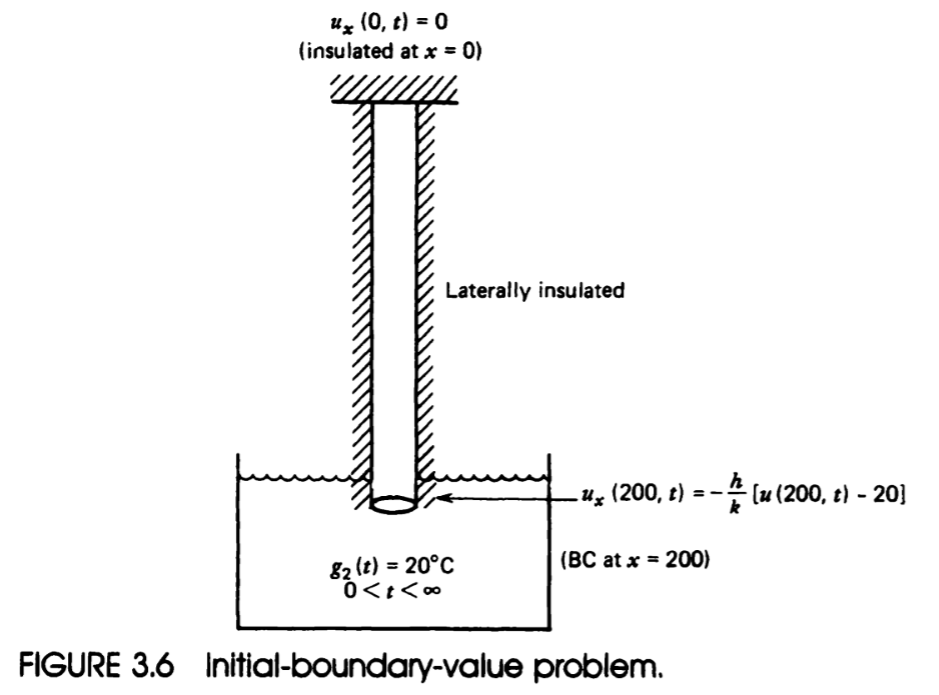
\includegraphics[scale=0.7]{type4.png}
\end{figure}

So, the IBVP is
\begin{align*}
\begin{cases*}
u_t = \alpha^2 u_xx\\
u_x(t,L) = 0\\
u_x(t,0) = -\lambda(u(t) - g_1(t)) \forall t > 0\\
u(0,x) = u_0(x) \forall 0\leq x \leq L
\end{cases*}
\end{align*}

\subsection{Derivation of the Heat Equation}
\begin{figure}[h!]
	\centering
	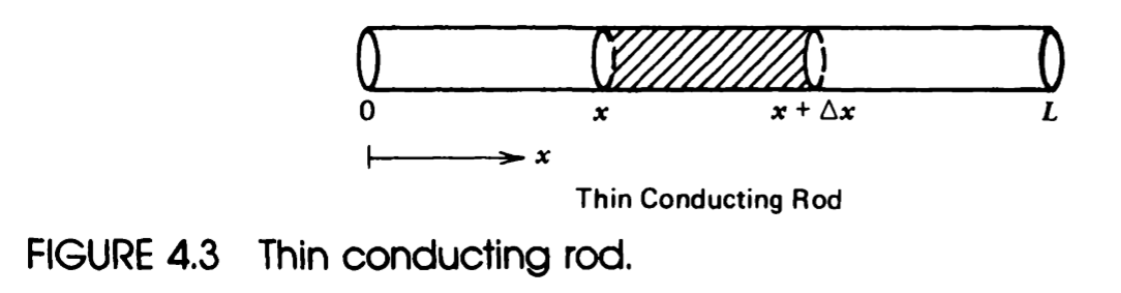
\includegraphics[scale=0.3]{heat.png}
\end{figure}
Main idea: Conservation of (Heat) Energy. Assumptions:
\begin{enumerate}
	\item The rod is a thermally homogeneous material 
	\item The temperature is constant across all cross-sections
	\item The rod is laterally insulated (no heat loss laterally)
\end{enumerate}
Using conservation of energy, we have the following: the change in thermal energy in the cross section $x$ to $x+\Delta x$ should be equal to the flux of the heat through the ``ends'' at $x$ and $x+\Delta x$ plus any external heat produced by some source (e.g. heat element). Some physical constants:
\begin{enumerate}
	\item $C$: thermal capacity of the rod
	\item $\rho$: density of the material of the rod
	\item $A$: area of cross section
	\item $k$: thermal conductivity
\end{enumerate}
Total heat inside is
\begin{align*}
\int_{x}^{\Delta x + x}c\rho A u(s,t)\,ds.
\end{align*}
The flux through the ends is
\begin{align*}
kA(u_x(x+\Delta x,t) - u_x(x, t)).
\end{align*}
The external energy is
\begin{align*}
A\int_x^{x+\Delta x}f(t,s)\,ds
\end{align*}
where $f(t,s)$ is the energy added at time $t$ and $x\leq s \leq x+\Delta x$. All together
\begin{align*}
\frac{d}{dt}\int_{x}^{\Delta x + x}c\rho A u(s,t)\,ds = kA(u_x(x+\Delta x,t) - u_x(x, t)) + A\int_x^{x+\Delta x}f(t,s)\,ds.
\end{align*}
Assuming that $u$ is nice enough, that
\begin{align*}
\frac{d}{dt}\int_{x}^{\Delta x + x}c\rho A u(s,t)\,ds = \int_{x}^{\Delta x + x}c\rho A u_t(s,t)\,ds.
\end{align*}
Also, the MVT for integrals says that if $G$ is continuous on the interval $[a,b]$ then $\exists c\in[a,b]$ such that
\begin{align*}
\int_a^b G(s)\,ds = G(c)(b-a).
\end{align*}
Therefore $\exists \chi \in [x,\Delta x]$ such that
\begin{align*}
\int_{x}^{\Delta x + x}c\rho A u_t(s,t)\,ds = c\rho A u_t(t,\chi)\Delta x
\end{align*}
and $\exists \eta \in [x,\Delta x]$ such that
\begin{align*}
A\int_x^{x+\Delta x}f(t,s)\,ds = Af(t,\eta)\Delta x.
\end{align*}
Combining all of these gives $\forall t > 0, \exists \chi,\eta \in [x,\Delta x]$ such that
\begin{align*}
c\rho Au_t(t,\chi)\Delta x &= kA(u_x(t,x+\Delta x) - u_x(t,x)) + Af(t,\eta)\Delta x\\
u_t(t,\chi) &= \frac{k}{\rho c}\frac{u_x(t,x+\Delta x) - u_x(t,x)}{\Delta x} + \frac{1}{c\rho}f(t,\eta).
\end{align*}
As $\Delta x \rightarrow 0$, $\eta,\chi \rightarrow x$
\begin{align*}
u_t(t,x) &= \frac{k}{\rho c}u_{xx}(x,t) + \frac{1}{c\rho}f(t,x)\\
u_t(t,x) &= \frac{k}{\rho c}u_{xx}(x,t) + F(t,x)\\
u_t(t,x) &= \alpha^2 u_{xx}(x,t) + F(t,x),
\end{align*}
where
\begin{align*}
\alpha^2 &= \frac{k}{\rho c}\\
F(t,x) &= \frac{1}{c\rho}f(t,x).
\end{align*}

\section{Separation of Variables - First method of solution}
Main idea: If the IBVP is posed on a rectangle, e.g. $t>0,x\in[0,L]$, and the PDE is linear, it is often the case that this method reduces the PDE into ODEs.
\subsection{Example: The heat equation}
\begin{align*}
u_t = \alpha^2 u_{xx}, t>0, x\in[0,1]
\end{align*}
We shall accompany this with so-called linear homogeneous BCs:
\begin{align*}
\alpha u(t,0) + \beta u_x(t,0) = 0\\
\gamma u(t,1) + \delta u_x(t,1) = 0.
\end{align*}
In fact, we specify further to assume
\begin{align*}
u(t,0)=0=u(t,1)\forall t > 0.
\end{align*}
We make an ansatz that solutions are of the form
\begin{align*}
u(t,x) = T(t)X(x).
\end{align*}
(Maybe not solutions but builidng blocks of solutions). 






























\end{document}
